\documentclass[11pt]{article}
\usepackage{lscape}
\usepackage{graphics}
\usepackage{graphicx}
\usepackage{color}
\usepackage{slashbox}
\usepackage{amsmath}
%\usepackage{times}
\usepackage{overcite}
\usepackage{endnotes}
\usepackage{geometry}
\geometry{letterpaper,tmargin=1in,bmargin=1in,lmargin=1in,rmargin=1in}
\usepackage{setspace}

\setlength{\oddsidemargin}{0cm} \setlength{\evensidemargin}{0cm}
\setlength{\textwidth}{6.5in} %\addtolength{\textheight}{2cm}
\setlength{\textheight}{9in} %\addtolength{\textheight}{2cm}
%\linespread{2}
\renewcommand{\thefootnote}{\fnsymbol{footnote}}

\begin{document}

\begin{figure}[htb!]
\begin{minipage}[c][60mm]{0.40\linewidth}
%\centering
%\vspace{8 mm}
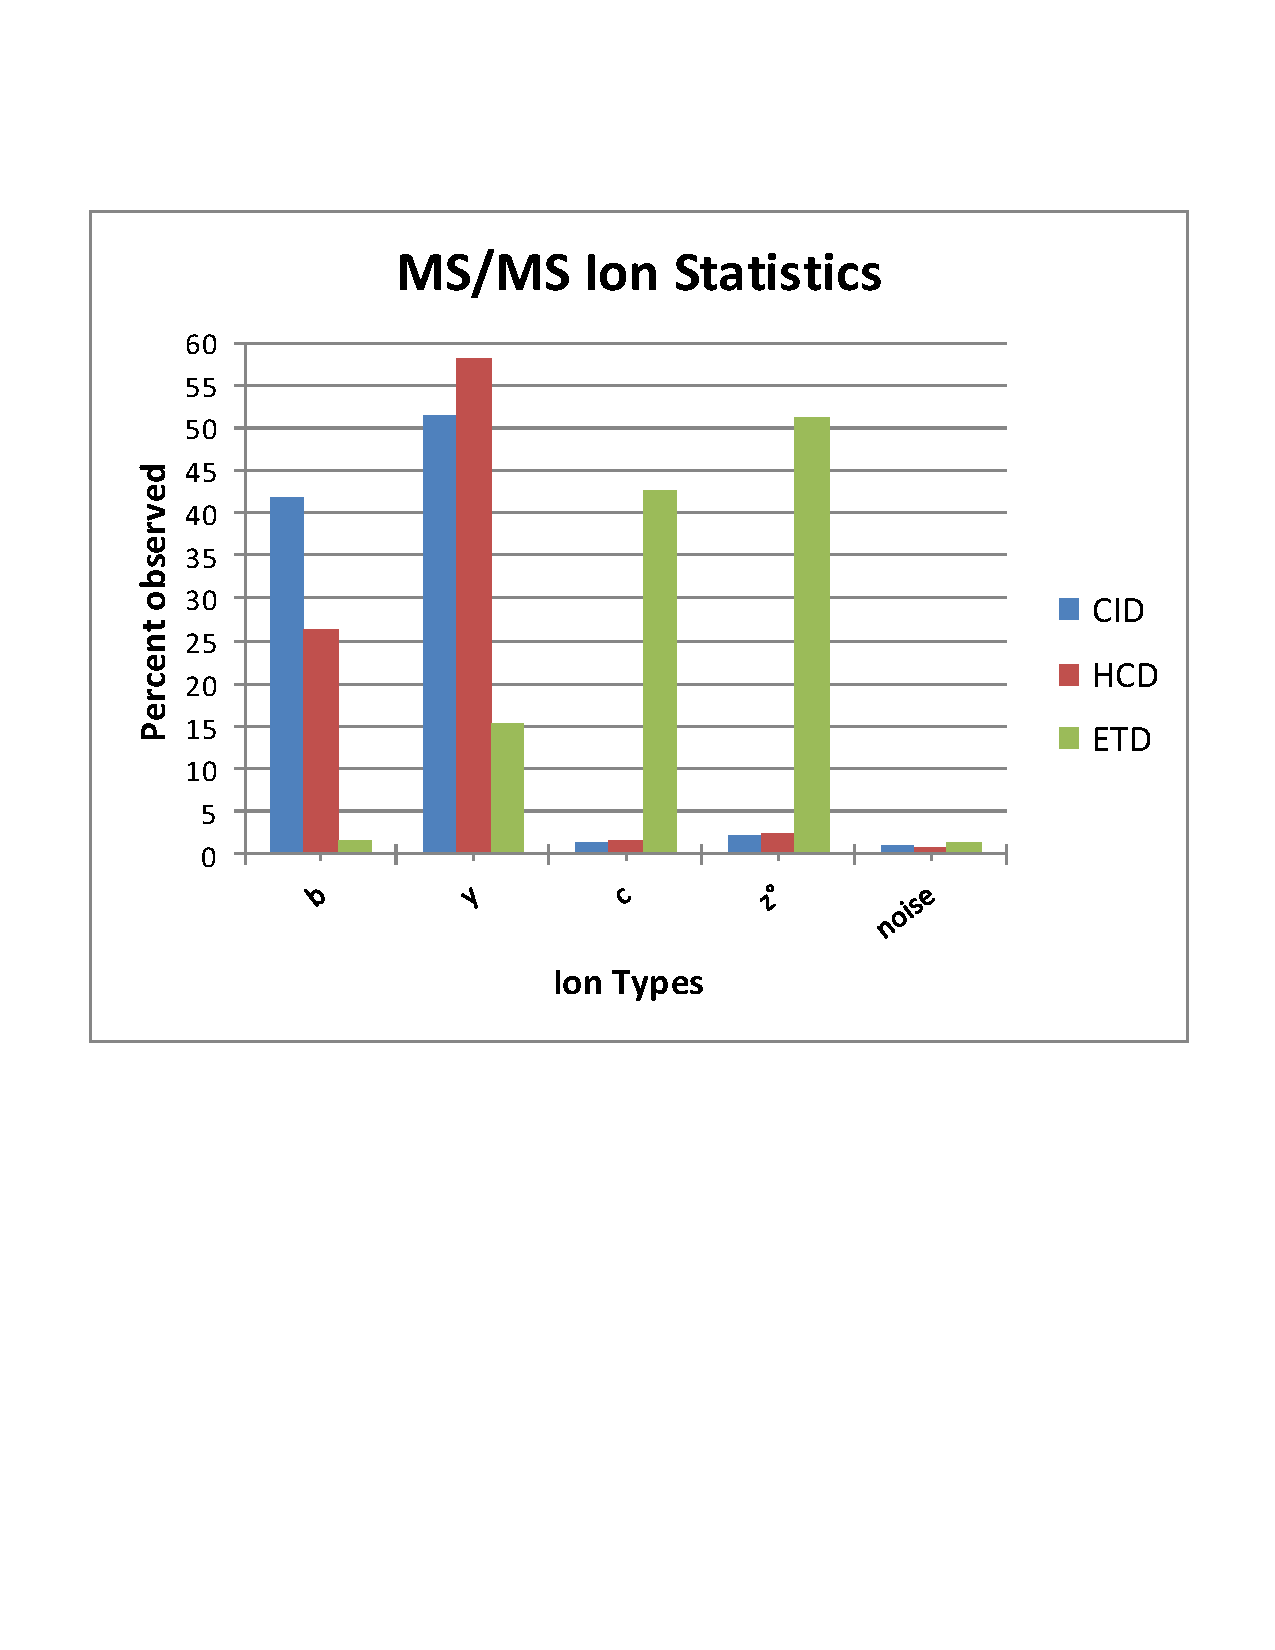
\includegraphics[scale=0.35]{Heck_ion_stats}
\end{minipage}
\begin{minipage}[c][60mm]{0.60\linewidth}
%\centering
%\vspace{45 mm}
\begin{tabular}{rccccc}
    & \multicolumn{5}{c}{Peptide Breaks}\\
\cline{2-6}
Prec. Charge  & $2$ & $3$ & $4$ & $5$ & All \\
\# Unique Pep. & 4361 & 2873 & 712 & 87 & 8037 \\
CID & 72.3 & 45.7 & 32.2 & 25.7 & 55.8\\
HCD & 74.1 & 54.0 & 34.9 & 27.1 & 60.3\\
ETD & 64.1 & 63.6 & 55.9 & 40.4 & 62.4\\
CID/HCD & 83.9 & 61.9 & 42.5 & 33.4 & 69.0\\
CID/ETD & 88.9 & 80.7 & 70.7 & 56.5 & 82.8\\
HCD/ETD & 89.1 & 84.3 & 72.1 & 57.4 & 84.4\\
CID/HCD/ETD & 93.2 & 86.8 & 75.4 & 61.1 & 87.8\\
\end{tabular}
\end{minipage}
\end{figure}

\end{document}
